\documentclass{article}
\usepackage[includeheadfoot,margin=1.0in]{geometry}
\usepackage{amsfonts}
\usepackage{amsmath}
\usepackage{amssymb}
\usepackage{fancyhdr}
\usepackage{hyperref}
\usepackage{graphicx}

\title{Software Requirements Specification}
\author{Team USA\\ Software Engineering: Fall 2015\\ Sam Houston State University}

\pagestyle{fancy}
\fancyhead[LE,RO]{SRS}
\fancyhead[RE,LO]{\leftmark}
\fancyfoot[RE,LO]{}
\renewcommand{\headrulewidth}{2pt}
\renewcommand{\thefootnote}{[\arabic{footnote}]}
\begin{document}
% Generate Title
\maketitle
\newpage

% Generate Table of Contents
\tableofcontents
\newpage

%Begin Section 1
\section{Introduction}
	\subsection{Purpose}
		Last Night in AB1 is a point and click, two-dimensional game taking place in AB1 on the Sam Houston State University campus. The player takes the role of a student, who must turn in a project before the midnight deadline, but there are a large number of obstacles standing in his or her way. 
		
		The game is survival horror themed, and the player is required to navigate through AB1 by collecting a series of items, which are randomly scattered throughout the various scenes. A scene consists of a photograph of a given room or hallway, where regions are defined as click-able by their distinctive art style. These regions can be interacted with to collect items or solve puzzles to progress through the game.
	
	\subsection{Document Conventions}
		\begin{itemize}
			\item Footnotes indicate that the reader should reference another section or subsection within the SRS to find additional information, as specified in the applicable footnote.
			\item Feature Priority
			\begin{itemize}
				\item \textbf{Critical} features are those without which the software will not function. 
				\item \textbf{High} priority features are those without which the software will function, but the overall quality and user experience will be severely affected. 
				\item \textbf{Moderate} priority features are those without which the software will function as expected, but user convenience features such as error logging or saving may be non-functional or otherwise affected. 
				\item \textbf{Low} priority features are those without which the software will function as expected with a fully developed user experience, but the software may lack perceived ``polish'' or completeness. 
			\end{itemize}
		\end{itemize}
	
	\subsection{Intended Audience and Reading Suggestions}
		This document is intended for developers, project managers, and testers. The remainder of this document contains the necessary information to design and implement the project. It includes the intended inputs and outputs of the entire system.
	
	\subsection{Product Scope}
		The objective of this project is to provide an entertaining and educational experience to the user-base consisting primarily of SHSU students. The final product should be maintainable and modifiable to allow the addition of game scenes and puzzles.
	
	\subsection{References}
		For textures:
		\begin{itemize}
			\item RFC2083 -- PNG (Portable Network Graphics) Specification, Version 1.0\\ \url{https://tools.ietf.org/html/rfc2083}
		\end{itemize}
    For fonts:
    \begin{itemize}
      \item TTF (TrueType Font) Specification\\ \url{https://www.microsoft.com/typography/tt/ttf_spec/ttch02.doc}
    \end{itemize}
		For audio:
		\begin{itemize}
			\item .WAV File Specification\\ \url{http://www-mmsp.ece.mcgill.ca/Documents/AudioFormats/WAVE/WAVE.html}
		\end{itemize}
% End Section 1, begin Section 2
\section{Overall Description}
	\subsection{Product Perspective}
		This is a standalone product that does not interface with other existing products
	
	\subsection{Product Functions}
		Major Functions:\footnote{See Section 7, Appendix A, Subsection 7.1, Figure. 1 for the appropriate data flow diagram.}
		\begin{itemize}
			\item Accept keyboard and mouse input 
			\item Render text and images onto program window
			\item Provide basic lighting and blending visual effects
			\item Play continuous background music and temporary sound effects simultaneously
			\item Read data files which specify game scenery and behavior
			\item Write data files to save game checkpoints and high scores
		\end{itemize}
	
	\subsection{User Classes and Characteristics}
		The game is playable by students and faculty alike, without any prior video game experience. It is intended to provide an entertaining experience given that the user has an understanding of culture in the Computer Science Department. 
	
	\subsection{Operating Environment}
		Since the target audience consists of all students in the Computer Science department at SHSU, all major platforms should be supported. \bigskip \\
		Platforms:
		\begin{itemize}
			\item Windows 7+
			\item Linux (Kernel 3.1+)
			\item Mac OS X 10.6+
		\end{itemize}
	
	\subsection{Design and Implementation Constraints}
		Requirements:
		\begin{itemize}
			\item Capable of rendering multiple layers of images simultaneously
			\item The ability to play multiple audio samples simultaneously (multi-threaded)
			\item The ability to store player progress on the disk to resume the game
		\end{itemize}
		Constraints:
		\begin{itemize}
			\item Each frame of the game must be rendered within an approximate 16.67ms frame time, to ensure the game displays at 60 frames per second on capable hardware.
		\end{itemize}
	
	\subsection{User Documentation}
		Included Documentation:
		\begin{itemize}
			\item A document is provided with the game files with instructions on how to launch the game
			\item When the game is started, an in-game screen is displayed to provide basic instructions
		\end{itemize}
	
	\subsection{Assumptions and Dependencies}
		User Assumptions:
		\begin{itemize}
			\item The user has reasonably modern hardware
			\item The user has a functioning EN-US keyboard and a standard two-button mouse
			\item The user is capable of reading the English language
		\end{itemize}
%End Section 2, begin Section 3
\section{External Interface Requirements}
	\subsection{User Interfaces}
		The main user interface will consist of the video display for output and the keyboard and mouse for user input. The following inputs are required:
		\begin{itemize}
			\item Mouse click
				\begin{itemize}
					\item Navigate main menu
					\item Move between scenes in the game
					\item Interact with objects in each scene
					\item Display the next sequence of on-screen text when required
				\end{itemize}
			\item Audio/video Output
				\begin{itemize}
					\item Main menu
					\begin{itemize}
						\item Background image
						\item Buttons - new game, load game, quit
						\begin{itemize}
							\item New Game (overwrites one of three available slots)
							\item Load Game (loads a game from one of three available slots)
							\item Quit (terminates program)
						\end{itemize}
					\end{itemize}
					\item Game play
					\begin{itemize}
						\item Scene image - an image simulating the player's view in AB1
						\item Interactive artwork - objects in the scene image that can be interacted with by clicking
						\item Characters - non-playable characters (NPCs) that operate independently of the player to stimuli in its environment. 
					\end{itemize}
					\item Text boxes
					\begin{itemize}
						\item Capable of displaying the full ASCII character set
						\item Communicate messages or other information to the player
					\end{itemize}
				\end{itemize}
			\end{itemize}
		Sample user interface:\\
		\begin{center}
			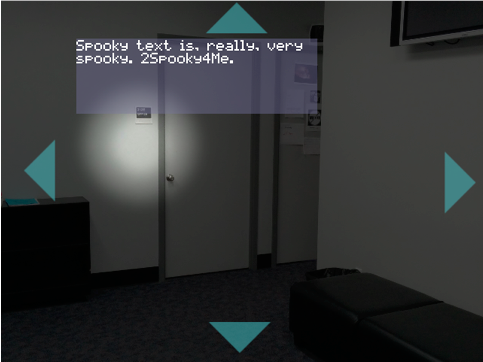
\includegraphics[scale=0.75]{SampleScreen}
		\end{center}
	\subsection{Hardware Interfaces}
		Required Interfaces:
		\begin{itemize}
			\item Standard 2-button mouse with scroll wheel
			\item Monitor or display capable of a minimum resolution of 1366 x 768 pixels
			\item Audio card capable of 16-bit PCM audio
		\end{itemize}
	\subsection{Communication Interfaces}
		There are no external communication interfaces, as this product does not utilize a network connection. 
% End section 3, begin Section 4
\section{System Features}
	\subsection{Video}
		\subsubsection{Description and Priority}
			The video subsystem should be capable of loading multiple PNG images into memory and converting them into textures that can be displayed to the user as the game environment.
      \footnote{See section 1, subsection 1.5, ``For Video:'' of this SRS for information on the PNG file specification.}
      Further, it should be capable of rendering ASCII text onto the screen by utilizing the given TrueType Font file.
      \footnote{See section 1, subsection 1.5, ``For Fonts:'' of this SRS for information on the TTF file specification.}\\
      \bigskip\\
			\textbf{Priority: Critical}
		\subsubsection{Stimulus/Response Sequences}
			Each level file contains the resources needed for each level. Combined with user input, the engine processes this information and determines video textures to load for display. These textures are then sent as output and displayed to the user. 
		\subsubsection{Functional Requirements}
			Textures should be generated from .PNG files. Text to display on screen should be generated through .TTF files.
	\subsection{Audio}
		\subsubsection{Description and Priority}
			The audio subsystem should be capable of loading multiple WAV format files into memory, which can then be played through the PC speakers. Further, the system should be able to stream one audio file from disk that can be continuously looped.\footnote{See section 1, subsection 1.5, ``For Audio:'' of this SRS for information on the WAV file specification.}\bigskip \\
			\textbf{Priority: Critical}
		\subsubsection{Stimulus/Response Sequences}
			Each level file contains the resources needed for each level. Combined with user input, the engine processes this information and determines the appropriate audio files to load. The audio generated from these files is sent as output to the attached or built-in speakers and heard by the user.
		\subsubsection{Functional Requirements}
			Audio should be generated from .WAV files. 
	\subsection{User Input}
		\subsubsection{Description and Priority}
			User input should be generated from an attached two-button, standard computer mouse. It will consist of cursor movement and position, or mouse button presses. For cursor movement and positioning, the system will expect a series of $(X, Y)$ coordinate pairs (integers) to be polled from the mouse input for each frame. This position will start in the top left corner of the game window. The vertical position will extend downward as the value of $Y$ increases, while the horizontal position will extend to the right as the value of $X$ increases. For button presses, the system should utilize a numerical integer value to represent which mouse button was pressed, so it can respond accordingly. \bigskip \\
			\textbf{Priority: Critical}
		\subsubsection{Stimulus/Response Sequences}
			Cursor position should be checked and stored for each rendered frame. This data should be used to determine appropriate in-game responses by entities or background objects that detect cursor movement. Mouse button clicks should be listened for and detected when they occur. This data should be used to determine appropriate in-game responses by entities or background objects that respond to button clicks. 
		\subsubsection{Functional Requirements}
			The system expects a mouse capable of at least two individual button presses, and capable of general cursor movement. The system should poll the mouse for cursor movements and button presses every frame. 
	\subsection{Game Levels}
		\subsubsection{Description and Priority}
			Level files will be plain ASCII text format, and will be utilized to specify what each level of the game will consist of and how it will behave. \bigskip \\
			\textbf{Priority: Critical}
		\subsubsection{Stimulus/Response Sequences}
			Level files should be provided to the game engine at level initialization. Level files should be pre-processed, and the appropriate level data output sent as input to the game engine.
		\subsubsection{Functional Requirements}
			Each level file should consist of a header, which contains an iteration of resources, followed by an iteration of scenes. The header will state which resources need to be loaded into memory and will assign the resources a unique identifier for the duration of the level's existence. These resources will then be utilized by the iteration of scenes in the body of the level file.
			 Each scene will:
			 \begin{itemize}
			 	\item Have a unique identifier
				\item Specify a background image to display
				\item Provide an iteration of actors\footnote{See the following subsection titled ``Actors'' for further information} that should be created and interacted with in the scene \bigskip
			\end{itemize}
	\subsection{Actors}
		\subsubsection{Description and Priority}
			An actor will provide a pre-defined interaction with the user, such as performing an action when the cursor is hovered over them or when they are clicked on. Each actor should be one line/record in the level file and should have a standard format such that actors can be iterated over.\footnote{See Section 8, Appendix B, Subsection 8.2 for the applicable data structure diagram} \bigskip \\
			\textbf{Priority: High}
		\subsubsection{Stimulus/Response Sequences}
			Actors will activate whenever interacted with by the user. The response sequences will vary depending on the type of actor that is interacted with. For example, an entity might scuttle horizontally across the screen when the actor detects that the cursor coordinates coincide with that actor's position. Another actor may respond when mouse button input is detected. 
		\subsubsection{Functional Requirements}
			Actors should be able to respond to user input, whether that input is a mouse button press or cursor movement. 
	\subsection{Multi-Threaded I/O}
		\subsubsection{Description and Priority}
			After reaching a specific checkpoints in the game, a worker thread should be spawned that will automatically save the user's progress in the background. Multi-threading this process prevents gameplay from being interrupted while the save file is written. \bigskip \\
			\textbf{Priority: Medium}
		\subsubsection{Stimulus/Response Sequences}
			This feature activates when the user enters a pre-defined area. For example, the beginning of a level. 
		\subsubsection{Functional Requirements}
			Attempt to open the save file and write progress. The feature will generate an error in the case of a failure. 
	\subsection{Error Handling}
		\subsubsection{Description and Priority}
			The program should ignore any unanticipated keyboard/mouse inputs. In the event that an error occurs in any other subsystem, the error should write a description of the issue in the log file. \bigskip \\
			\textbf{Priority: Medium}
		\subsubsection{Stimulus/Response Sequences}
			This feature activates whenever an unexpected event occurs that impacts logical processing, and responds by writing a report of the error to the log file. 
		\subsubsection{Functional Requirements}
			The message should be logged to an external log file. It should be descriptive enough to fully convey the error, but concise enough as to not overload the person reading the log with information.\footnote{See Section 8, Appendix B, Subsection 8.3 for the applicable data structure diagram.}
	\subsection{Loading and Saving Progress}
		\subsubsection{Description and Priority}
			The system should output a save file whenever the user wishes to quit the game in the middle of a play-through.  \bigskip \\
			\textbf{Priority: Medium}
		\subsubsection{Stimulus/Response Sequences}
			This feature can be activated automatically upon reaching certain in game areas, or can be activated manually by the user if they wish to stop the game before it has been completed. The game engine will output a save file to be stored on disk. Upon resuming the game, the game engine will attempt to load the appropriate save file as an input and resume where the user left off. 
		\subsubsection{Functional Requirements}
			The save file should consist of the applicable save slot, the player's inventory, and the current scene ID, such that it can be used as input whenever the user wishes to resume from their previous save point.\footnote{See Section 8, Appendix B, Subsection 8.4 for the applicable data structure diagram.}
% End Section 4, Begin Section 5
\section{Other Nonfunctional Requirements}
	\subsection{Performance Requirements}
		Frames should be rendered approximately every 16.67 milliseconds, in order to insure a final frame rate of 60 frames per second on capable, modern hardware with sufficient resources. A frame rate of 60 frames per second is a very common, almost standard, render rate for modern video games. 
	\subsection{Safety Requirements}
		Certain scenes or areas in the product may contain flashing lights or fast moving objects that could affect the health of sensitive individuals. Persons prone to photosensitive seizures should not be exposed to gameplay visuals during development, testing, or after release. 
	\subsection{Security Requirements}
		There are no specific security requirements in this product, other than the typical expectation that the product will not be able to access (read/write) unallocated memory or data. 
	\subsection{Software Quality Attributes}
		The game engine developed should be adaptable enough to perform as a base to any point-and-click game with little-to-no modification. The details of the game will be specified in configuration files and text-based files, which will allow for the creation of additional levels, scenes, etcetera, without modifying the program itself. To allow for easy maintenance and modification of the engine, the game logic will be separate from the video, audio, and I/O modules. This design will allow the engine to be utilized for other types of two-dimensional games with minimal modification to the code base. 
% End Section 5, begin Section 6
\section{Other Requirements}
	\subsection{Re-use Objectives}
		The game engine should be designed in such a way that it can be used to build further two-dimensional point-and-click style games with minimal modification. Further, the audio and video modules are designed to be reusable as standalone modules that can be imported into future projects with no modifications to code.
% End Section 5, Begin Appendix A
\section{Appendix A: Analysis Models}
	\subsection{General Data Flow Diagram}
		\begin{center}
			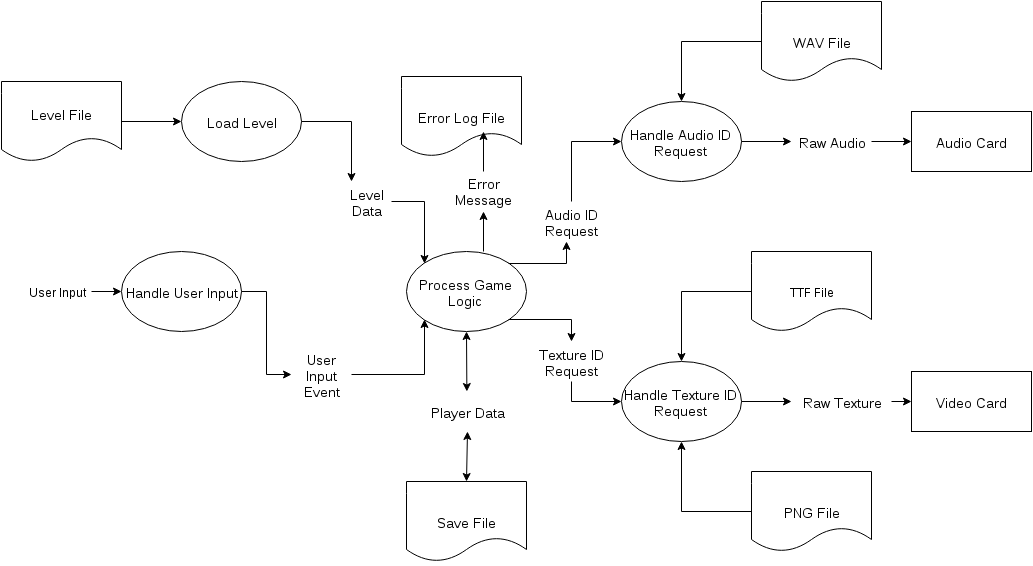
\includegraphics[scale=0.45]{DataFlow}
		\end{center}
		Data Flow:
		\begin{enumerate}
      \item Player data states which level to load from the save manager if a previous save is available. Otherwise, the default level is selected
			\item A level file is loaded, generating level data which is passed to the engine
			\item The engine sends Load Audio requests to the audio player, instructing it to load raw audio from the appropriate audio files
			\item The engine sends Load Video requests to the video display, instructing it to create textures from the appropriate image/font files
			\item Cursor coordinates and mouse clicks are processed into user input events, which are passed to the engine
			\item The engine processes the mouse input it receives and generates the appropriate audio and video rendering requests
      \item The generated audio and video rendering requests are sent to their respective modules, which present the loaded material
			\item Audio and video cards are the final output, and are what the user sees as reactions in the game world to the user's own input
      \item In the event of an error, the message is written to the log file.
		\end{enumerate}
% End Appendix A, begin Appendix B
\section{Appendix B: Input \& Output Data Structure Diagrams}
	\subsection{User Input}
		\begin{center}
			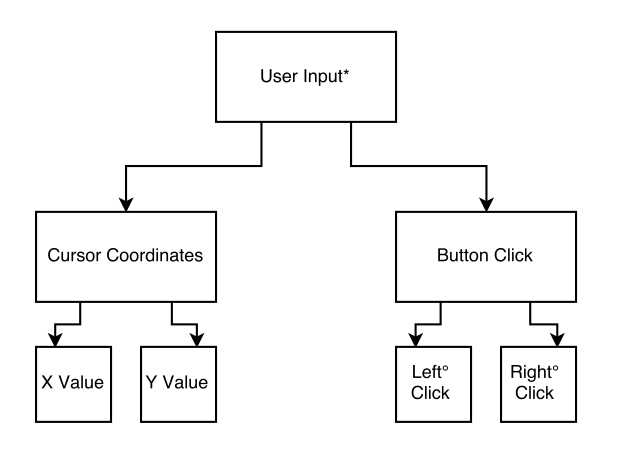
\includegraphics{UserInput}
		\end{center}
	\subsection{Level File}
		\begin{center}
			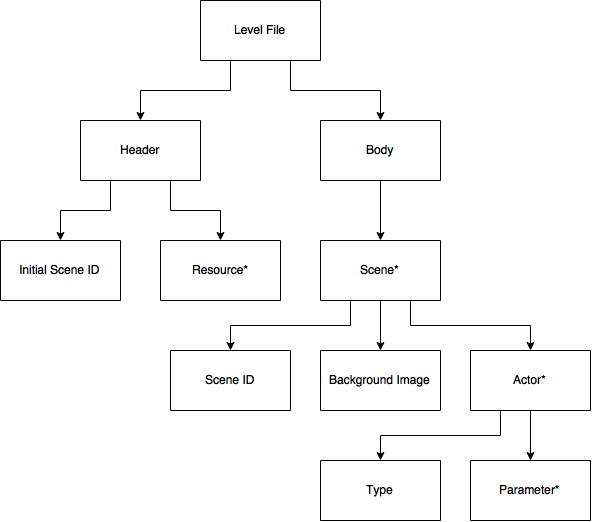
\includegraphics[scale=0.75]{LevelFile}
		\end{center}
	\subsection{Error File}
		\begin{center}
			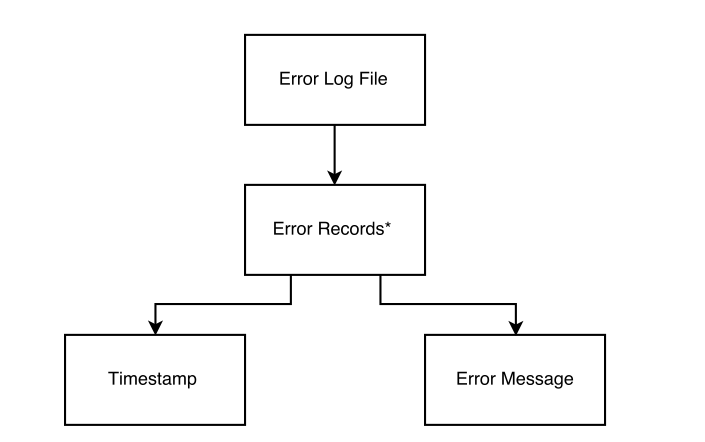
\includegraphics{ErrorFile}
		\end{center}
	\subsection{Save File}
		\begin{center}
			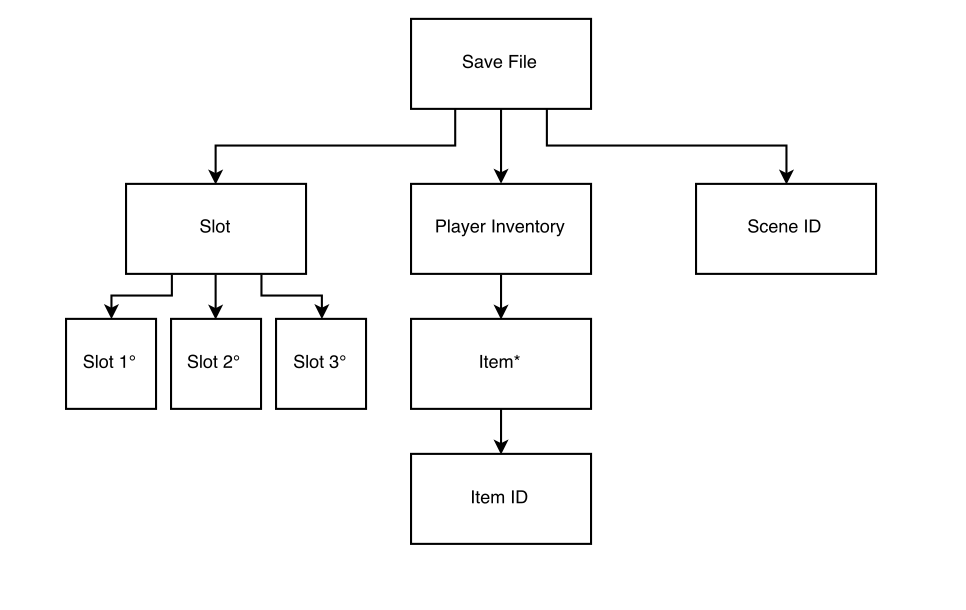
\includegraphics{SaveFile}
		\end{center}
% End Appendix B, end document
\end{document}
